\documentclass[]{article}
\usepackage{lmodern}
\usepackage{amssymb,amsmath}
\usepackage{ifxetex,ifluatex}
\usepackage{fixltx2e} % provides \textsubscript
\ifnum 0\ifxetex 1\fi\ifluatex 1\fi=0 % if pdftex
  \usepackage[T1]{fontenc}
  \usepackage[utf8]{inputenc}
\else % if luatex or xelatex
  \ifxetex
    \usepackage{mathspec}
  \else
    \usepackage{fontspec}
  \fi
  \defaultfontfeatures{Ligatures=TeX,Scale=MatchLowercase}
\fi
% use upquote if available, for straight quotes in verbatim environments
\IfFileExists{upquote.sty}{\usepackage{upquote}}{}
% use microtype if available
\IfFileExists{microtype.sty}{%
\usepackage{microtype}
\UseMicrotypeSet[protrusion]{basicmath} % disable protrusion for tt fonts
}{}
\usepackage[margin=1.5cm]{geometry}
\usepackage{hyperref}
\hypersetup{unicode=true,
            pdftitle={Calculus for Stat 343},
            pdfborder={0 0 0},
            breaklinks=true}
\urlstyle{same}  % don't use monospace font for urls
\usepackage{color}
\usepackage{fancyvrb}
\newcommand{\VerbBar}{|}
\newcommand{\VERB}{\Verb[commandchars=\\\{\}]}
\DefineVerbatimEnvironment{Highlighting}{Verbatim}{commandchars=\\\{\}}
% Add ',fontsize=\small' for more characters per line
\usepackage{framed}
\definecolor{shadecolor}{RGB}{248,248,248}
\newenvironment{Shaded}{\begin{snugshade}}{\end{snugshade}}
\newcommand{\KeywordTok}[1]{\textcolor[rgb]{0.13,0.29,0.53}{\textbf{#1}}}
\newcommand{\DataTypeTok}[1]{\textcolor[rgb]{0.13,0.29,0.53}{#1}}
\newcommand{\DecValTok}[1]{\textcolor[rgb]{0.00,0.00,0.81}{#1}}
\newcommand{\BaseNTok}[1]{\textcolor[rgb]{0.00,0.00,0.81}{#1}}
\newcommand{\FloatTok}[1]{\textcolor[rgb]{0.00,0.00,0.81}{#1}}
\newcommand{\ConstantTok}[1]{\textcolor[rgb]{0.00,0.00,0.00}{#1}}
\newcommand{\CharTok}[1]{\textcolor[rgb]{0.31,0.60,0.02}{#1}}
\newcommand{\SpecialCharTok}[1]{\textcolor[rgb]{0.00,0.00,0.00}{#1}}
\newcommand{\StringTok}[1]{\textcolor[rgb]{0.31,0.60,0.02}{#1}}
\newcommand{\VerbatimStringTok}[1]{\textcolor[rgb]{0.31,0.60,0.02}{#1}}
\newcommand{\SpecialStringTok}[1]{\textcolor[rgb]{0.31,0.60,0.02}{#1}}
\newcommand{\ImportTok}[1]{#1}
\newcommand{\CommentTok}[1]{\textcolor[rgb]{0.56,0.35,0.01}{\textit{#1}}}
\newcommand{\DocumentationTok}[1]{\textcolor[rgb]{0.56,0.35,0.01}{\textbf{\textit{#1}}}}
\newcommand{\AnnotationTok}[1]{\textcolor[rgb]{0.56,0.35,0.01}{\textbf{\textit{#1}}}}
\newcommand{\CommentVarTok}[1]{\textcolor[rgb]{0.56,0.35,0.01}{\textbf{\textit{#1}}}}
\newcommand{\OtherTok}[1]{\textcolor[rgb]{0.56,0.35,0.01}{#1}}
\newcommand{\FunctionTok}[1]{\textcolor[rgb]{0.00,0.00,0.00}{#1}}
\newcommand{\VariableTok}[1]{\textcolor[rgb]{0.00,0.00,0.00}{#1}}
\newcommand{\ControlFlowTok}[1]{\textcolor[rgb]{0.13,0.29,0.53}{\textbf{#1}}}
\newcommand{\OperatorTok}[1]{\textcolor[rgb]{0.81,0.36,0.00}{\textbf{#1}}}
\newcommand{\BuiltInTok}[1]{#1}
\newcommand{\ExtensionTok}[1]{#1}
\newcommand{\PreprocessorTok}[1]{\textcolor[rgb]{0.56,0.35,0.01}{\textit{#1}}}
\newcommand{\AttributeTok}[1]{\textcolor[rgb]{0.77,0.63,0.00}{#1}}
\newcommand{\RegionMarkerTok}[1]{#1}
\newcommand{\InformationTok}[1]{\textcolor[rgb]{0.56,0.35,0.01}{\textbf{\textit{#1}}}}
\newcommand{\WarningTok}[1]{\textcolor[rgb]{0.56,0.35,0.01}{\textbf{\textit{#1}}}}
\newcommand{\AlertTok}[1]{\textcolor[rgb]{0.94,0.16,0.16}{#1}}
\newcommand{\ErrorTok}[1]{\textcolor[rgb]{0.64,0.00,0.00}{\textbf{#1}}}
\newcommand{\NormalTok}[1]{#1}
\usepackage{graphicx,grffile}
\makeatletter
\def\maxwidth{\ifdim\Gin@nat@width>\linewidth\linewidth\else\Gin@nat@width\fi}
\def\maxheight{\ifdim\Gin@nat@height>\textheight\textheight\else\Gin@nat@height\fi}
\makeatother
% Scale images if necessary, so that they will not overflow the page
% margins by default, and it is still possible to overwrite the defaults
% using explicit options in \includegraphics[width, height, ...]{}
\setkeys{Gin}{width=\maxwidth,height=\maxheight,keepaspectratio}
\IfFileExists{parskip.sty}{%
\usepackage{parskip}
}{% else
\setlength{\parindent}{0pt}
\setlength{\parskip}{6pt plus 2pt minus 1pt}
}
\setlength{\emergencystretch}{3em}  % prevent overfull lines
\providecommand{\tightlist}{%
  \setlength{\itemsep}{0pt}\setlength{\parskip}{0pt}}
\setcounter{secnumdepth}{0}
% Redefines (sub)paragraphs to behave more like sections
\ifx\paragraph\undefined\else
\let\oldparagraph\paragraph
\renewcommand{\paragraph}[1]{\oldparagraph{#1}\mbox{}}
\fi
\ifx\subparagraph\undefined\else
\let\oldsubparagraph\subparagraph
\renewcommand{\subparagraph}[1]{\oldsubparagraph{#1}\mbox{}}
\fi

%%% Use protect on footnotes to avoid problems with footnotes in titles
\let\rmarkdownfootnote\footnote%
\def\footnote{\protect\rmarkdownfootnote}

%%% Change title format to be more compact
\usepackage{titling}

% Create subtitle command for use in maketitle
\newcommand{\subtitle}[1]{
  \posttitle{
    \begin{center}\large#1\end{center}
    }
}

\setlength{\droptitle}{-2em}

  \title{Calculus for Stat 343}
    \pretitle{\vspace{\droptitle}\centering\huge}
  \posttitle{\par}
    \author{}
    \preauthor{}\postauthor{}
    \date{}
    \predate{}\postdate{}
  
\usepackage{booktabs}

\begin{document}
\maketitle

\section{Pre-Calculus}\label{pre-calculus}

\subsubsection{Sums}\label{sums}

You can factor anything that doesn't depend on the summation index out
of a sum:

\[\sum_{i = 1}^n c x_i = (c x_1 + c x_2 + \cdots + c x_n) = c(x_1 + x_2 + \cdots + x_n) = c \sum_{i = 1}^n x_i\]

\subsubsection{Products}\label{products}

You can factor anything that doesn't depend on the product index out of
a product, but you have to raise it to the power of the number of terms
in the product:

\[\prod_{i = 1}^n c x_i = (c x_1)(c x_2) \cdots (c x_n) = c^n \prod_{i = 1}^n x_i\]

\subsubsection{Logarithms and Exponents}\label{logarithms-and-exponents}

\(a\), \(b\), and \(c\) are real numbers, \(e \approx 2.718281828459\)
is Euler's number.

\(\log(a)\) is defined to be the number to which you raise \(e\) in
order to get \(a\): \(e^{\log(a)} = a\).

\(\log(e) = 1\)

\(\log(ab) = \log(a) + \log(b)\)

\(\log(a^b) = b \log(a)\)

\(\log(a/b) = \log(a) - \log(b)\)

\(a^b \cdot a^c = a^{b + c}\)

\subsubsection{Gamma Function}\label{gamma-function}

The Gamma (\(\Gamma\)) function is basically a continuous version of the
factorial. If \(a\) is an integer, then

\(\Gamma(a) = (a-1)!\)

If \(a\) is a real number, the \(\Gamma\) function is still defined, and
it's basically a smooth interpolation between the factorials of nearby
integers. There's a way to define the \(\Gamma\) function as an
integral, but we won't need to know that.

\newpage

\section{Differential Calculus in One
Variable}\label{differential-calculus-in-one-variable}

\subsubsection{Chain rule:}\label{chain-rule}

Suppose \(f\) and \(g\) are functions, and define \(h\) by
\(h(x) = f(g(x))\). Then \(h'(x) = f'(g(x)) \cdot g'(x)\)

\subsubsection{Derivative of a
polynomial:}\label{derivative-of-a-polynomial}

If \(a \neq 0\) then \(\frac{d}{dx} x^a = a x^{a-1}\)

Two special cases that come up a lot are \(a = -1\) and \(a = -2\):

If \(a = -1\) then
\(\frac{d}{dx} \frac{1}{x} = \frac{d}{dx} x^{-1} = -1 x^{-2} = \frac{-1}{x^2}\)

If \(a = -2\) then
\(\frac{d}{dx} \frac{1}{x^2} = \frac{d}{dx} x^{-2} = -2 x^{-3} = \frac{-2}{x^3}\)

\subsubsection{Derivative of an
exponential:}\label{derivative-of-an-exponential}

\(\frac{d}{dx} e^{x} = e^x\)

In combination with the chain rule, we get

\(\frac{d}{dx} e^{f(x)} = e^{f(x)} f'(x)\)

\subsubsection{Derivative of a
logarithm:}\label{derivative-of-a-logarithm}

\(\frac{d}{dx} \log(x) = \frac{1}{x}\)

In combination with the chain rule, we get

\(\frac{d}{dx} \log(f(x)) = \frac{1}{f(x)} f'(x)\)

\subsubsection{Finding maximum and minimum of a
function}\label{finding-maximum-and-minimum-of-a-function}

To find a maximum or minimum of a function \(f(x)\), we can often use
this procedure:

\begin{enumerate}
\def\labelenumi{\arabic{enumi}.}
\tightlist
\item
  Find a \textbf{critical point} \(x^*\) by setting the first derivative
  to 0 and solving for \(x\).
\item
  Verify that the critical point is a maximum or minimum; in this class,
  we will typically use the second derivative test to do this:

  \begin{enumerate}
  \def\labelenumii{\arabic{enumii}.}
  \tightlist
  \item
    If \(f''(x^*) > 0\) (at the critical point), the critical point is a
    \textbf{local minimum} of \(f\)
  \item
    If \(f''(x) > 0\) (at all values of \(x\)), the critical point is a
    \textbf{global minimum} of \(f\)
  \item
    If \(f''(x^*) < 0\) (at the critical point), the critical point is a
    \textbf{local maximum} of \(f\)
  \item
    If \(f''(x) < 0\) (at all values of \(x\)), the critical point is a
    \textbf{global maximum} of \(f\)
  \end{enumerate}
\end{enumerate}

Let's illustrate by finding an extreme point of the function
\(f(x) = 3x^2 - 12x + 14\) and seeing whether it is a local or global
minimum or maximum.

Step 1: Find a critical point

\[\frac{d}{dx} f(x) = \frac{d}{dx} 3x^2 - 12x + 14 = 6x - 12 = 0\]

Solving for \(x\), we find that \(x^* = 2\) is a critical point.

Step 2: Determine whether the critical point is a maximum or minimum,
and whether it is local or global

\[\frac{d^2}{dx^2} f(x) = \frac{d^2}{dx^2} 3x^2 - 12x + 14 = \frac{d}{dx} 6x - 12 = 6\]

Since the second derivative is positive for all values of \(x\), the
critical point \(x^* = 2\) is a global minimum of \(f\). Here's a
picture:

\begin{Shaded}
\begin{Highlighting}[]
\KeywordTok{library}\NormalTok{(ggplot2)}
\NormalTok{f <-}\StringTok{ }\ControlFlowTok{function}\NormalTok{(x) \{}
  \DecValTok{3}\OperatorTok{*}\NormalTok{x}\OperatorTok{^}\DecValTok{2} \OperatorTok{-}\StringTok{ }\DecValTok{12}\OperatorTok{*}\NormalTok{x }\OperatorTok{+}\StringTok{ }\DecValTok{14}
\NormalTok{\}}

\KeywordTok{ggplot}\NormalTok{(}\DataTypeTok{data =} \KeywordTok{data.frame}\NormalTok{(}\DataTypeTok{x =} \KeywordTok{c}\NormalTok{(}\OperatorTok{-}\DecValTok{5}\NormalTok{, }\DecValTok{9}\NormalTok{)), }\DataTypeTok{mapping =} \KeywordTok{aes}\NormalTok{(}\DataTypeTok{x =}\NormalTok{ x)) }\OperatorTok{+}
\StringTok{  }\KeywordTok{stat_function}\NormalTok{(}\DataTypeTok{fun =}\NormalTok{ f) }\OperatorTok{+}
\StringTok{  }\KeywordTok{geom_vline}\NormalTok{(}\DataTypeTok{xintercept =} \DecValTok{2}\NormalTok{)}
\end{Highlighting}
\end{Shaded}

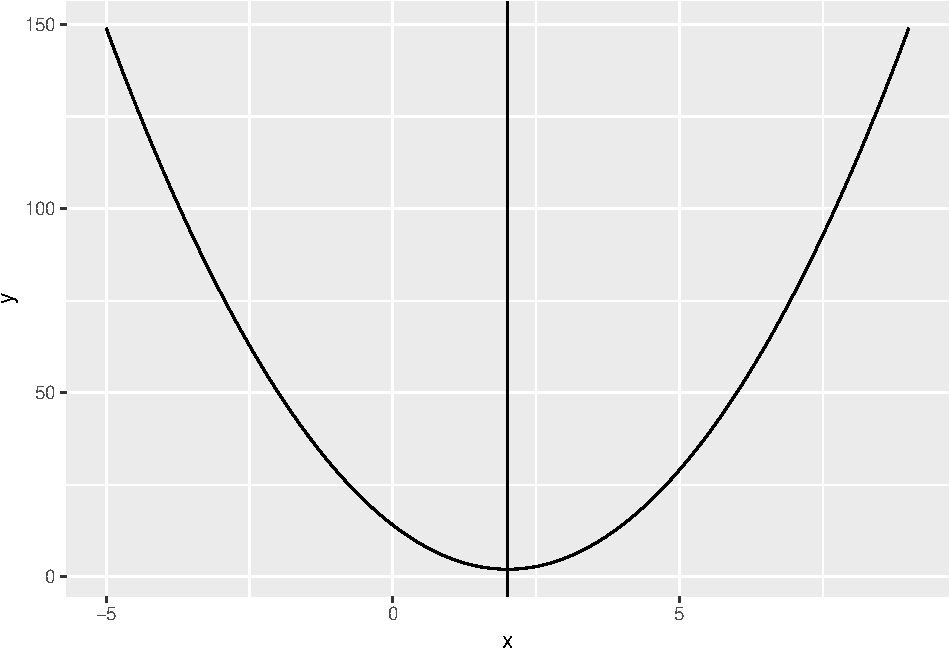
\includegraphics{calculus_files/figure-latex/unnamed-chunk-1-1.pdf}

\subsubsection{Taylor's Theorem}\label{taylors-theorem}

I adapted this statement of Taylor's theorem from Wikipedia:
\url{https://en.wikipedia.org/wiki/Taylor\%27s_theorem\#Taylor's_theorem_in_one_real_variable}

Let \(k \geq 1\) be an integer and suppose that the function
\(f: \mathbb{R} \rightarrow \mathbb{R}\) is \(k\) times differentiable
at the point \(a \in \mathbb{R}\). Define the \(k\)-th order polynomial
approximation to \(f\) centered at \(a\) by

\(P_k(x) = f(a) + f'(a) (x - a) + \frac{f''(a)}{2!} (x - a)^2 + \cdots + \frac{f^{(k)}(a)}{k!}(x - a)^k\)

Then there exists a function \(h_k: \mathbb{R} \rightarrow \mathbb{R}\)
such that:

\begin{itemize}
\item $f(x) = P_k(x) + h_k(x) (x - a)^k$ and
\item $\lim_{x \rightarrow a} h_k(x) = 0$
\end{itemize}

(You can get more specific about what the function \(h_k\) looks like
and rates of convergence to 0, but we don't need to do that.)

The main points are:

\begin{enumerate}
\def\labelenumi{\arabic{enumi}.}
\tightlist
\item
  For values of \(x\) near \(a\), the function \(f(x)\) can be well
  approximated by a polynomial, and the polynomial's coefficients can be
  obtained by the derivatives of \(f\).
\item
  The approximation is better if you use a higher degree polynomial.
\end{enumerate}

\newpage

As an example, let's approximate \(f(x) = e^{5x}\) by a second-order
Taylor polynomial centered at \(a = 1\). We will need the first and
second derivatives of \(f(x)\):

\begin{align*}
\frac{d}{dx} e^{5x} &= e^{5x} \cdot 5 \\
\frac{d^2}{dx^2} e^{5x} &= \frac{d}{dx} e^{5x} \cdot 5 = e^{5x} \cdot 25
\end{align*}

\begin{align*}
P_2(x) &= f(1) + f'(1) (x - 1) + \frac{f''(1)}{2} (x - 1)^2 \\
&= e^{5 \cdot 1} + 5 e^{5 \cdot 1}(x - 1) + \frac{25 e^{5 \cdot 1}}{2}(x - 1)^2
\end{align*}

The claim is that \(f(x)\) looks very similar to \(P_2(x)\) for values
of \(x\) near \(a = 1\). Let's verify with a picture:

\begin{Shaded}
\begin{Highlighting}[]
\KeywordTok{library}\NormalTok{(ggplot2)}
\NormalTok{f <-}\StringTok{ }\ControlFlowTok{function}\NormalTok{(x) \{}
  \KeywordTok{exp}\NormalTok{(}\DecValTok{5} \OperatorTok{*}\StringTok{ }\NormalTok{x)}
\NormalTok{\}}

\NormalTok{P_}\DecValTok{2}\NormalTok{ <-}\StringTok{ }\ControlFlowTok{function}\NormalTok{(x) \{}
  \KeywordTok{exp}\NormalTok{(}\DecValTok{5}\NormalTok{) }\OperatorTok{+}\StringTok{ }\DecValTok{5} \OperatorTok{*}\StringTok{ }\KeywordTok{exp}\NormalTok{(}\DecValTok{5}\NormalTok{) }\OperatorTok{*}\StringTok{ }\NormalTok{(x }\OperatorTok{-}\StringTok{ }\DecValTok{1}\NormalTok{) }\OperatorTok{+}\StringTok{ }\NormalTok{(}\DecValTok{25} \OperatorTok{*}\StringTok{ }\KeywordTok{exp}\NormalTok{(}\DecValTok{5}\NormalTok{)) }\OperatorTok{/}\StringTok{ }\DecValTok{2} \OperatorTok{*}\StringTok{ }\NormalTok{(x }\OperatorTok{-}\StringTok{ }\DecValTok{1}\NormalTok{)}\OperatorTok{^}\DecValTok{2}
\NormalTok{\}}

\NormalTok{temp_df <-}\StringTok{ }\KeywordTok{data.frame}\NormalTok{(}\DataTypeTok{x =} \KeywordTok{c}\NormalTok{(}\FloatTok{0.5}\NormalTok{, }\FloatTok{1.5}\NormalTok{))}
\KeywordTok{ggplot}\NormalTok{(}\DataTypeTok{data =}\NormalTok{ temp_df, }\DataTypeTok{mapping =} \KeywordTok{aes}\NormalTok{(}\DataTypeTok{x =}\NormalTok{x)) }\OperatorTok{+}
\StringTok{  }\KeywordTok{stat_function}\NormalTok{(}\DataTypeTok{fun =}\NormalTok{ f) }\OperatorTok{+}
\StringTok{  }\KeywordTok{stat_function}\NormalTok{(}\DataTypeTok{fun =}\NormalTok{ P_}\DecValTok{2}\NormalTok{, }\DataTypeTok{color =} \StringTok{"orange"}\NormalTok{)}
\end{Highlighting}
\end{Shaded}

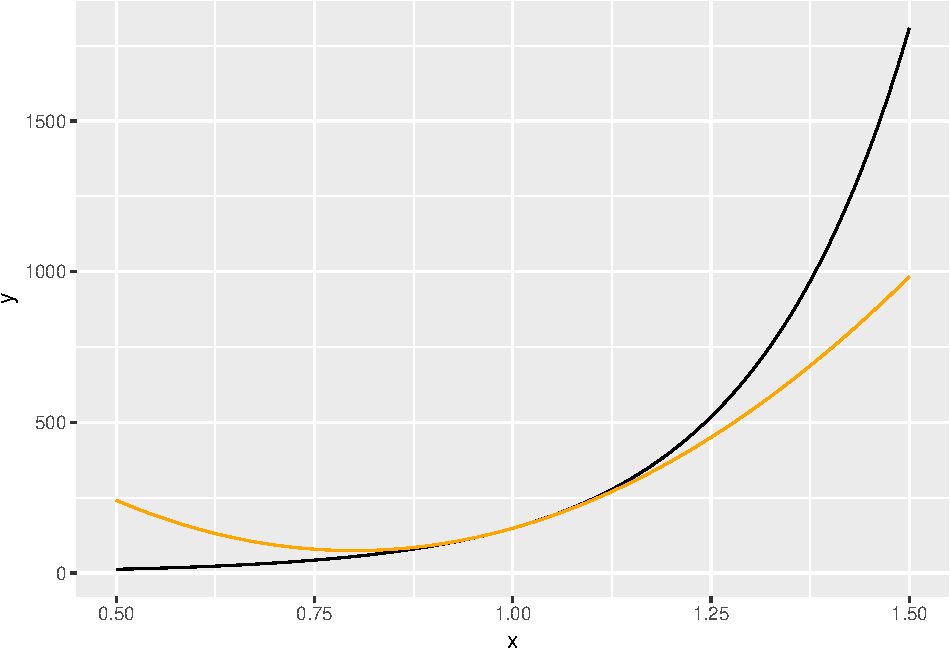
\includegraphics{calculus_files/figure-latex/unnamed-chunk-2-1.pdf}


\end{document}
